\documentclass[a4paper, 11pt]{scrreprt}
\usepackage[utf8]{inputenc}
\usepackage[ngerman]{babel}
\usepackage{amsfonts}   
\usepackage{amssymb}
\usepackage{amsmath}
\usepackage{amsthm}
\usepackage{enumitem}
\usepackage{geometry}
\usepackage{jurabib}
\usepackage{remreset}
\usepackage{tikz}
\usepackage{setspace}
\usepackage{graphicx}
\usepackage{minted}

\makeatletter
\@removefromreset{footnote}{chapter}
\makeatother

\jurabibsetup{
  authorformat=year,
  commabeforerest,
  ibidem=strict,
  citefull=first,
  see,
  titleformat=colonsep,
}

\renewcommand*{\jbauthorfont}{\textsc}
\renewcommand*{\biblnfont}{\scshape\textbf}
\renewcommand*{\bibfnfont}{\normalfont\textbf}

%AddTo\bibsgerman{%
%	\renewcommand*{\ibidemname}{Ibidem}
%	\renewcommand*{\ibidemmidname}{ibidem}
%}


\geometry{a4paper,left=25mm,right=25mm, top=25mm, bottom=25mm}
\parindent0pt

\begin{document}

\thispagestyle{empty}
\begin{center}
\Large{Universität Osnabrück}\\
\end{center}


\begin{center}
\Large{Fachbereich Mathematik/Informatik}
\end{center}
\begin{verbatim}





\end{verbatim}
\begin{center}
\textbf{\LARGE{Seminararbeit}}
\end{center}
\begin{verbatim}


\end{verbatim}
\begin{center}
\textbf{zum Seminar ``Programmiersprachen'' im Sommersemester 2011}
\end{center}
\begin{verbatim}
















\end{verbatim}

\begin{flushleft}
\begin{tabular}{lll}
\textbf{Thema:} & & Die Programmiersprache Ruby\\
& & \\
& & \\
& & \\
& & \\
\textbf{eingereicht von:} & & Manuel Schwarz \flq{}manschwa@uos.de\frq{}\\
\textbf{Matrikelnr.:} & & 935488\\
& & \\
& & \\
\textbf{eingereicht am:} & & 15. Juni 2011\\
& & \\
& & \\
\textbf{Betreuerin:} & & Frau Dr. rer. nat. Jutta Göers 
\end{tabular}
\end{flushleft}

\newpage


\onehalfspacing
\thispagestyle{empty}

\tableofcontents
\newpage
\listoffigures
\newpage

\chapter{Einleitung}
Die vorliegende Seminararbeit entstand im Rahmen des Seminars 
``Programmiersprachen'' an der Universität Osnabrück im Sommersemester 2011
unter der Leitung von Dr. rer. nat. Jutta Göers als Ausarbeitung eines 
45-minütigen Vortrages.\\
Das Seminar hatte zum Ziel Einführungen in eine Reihe von Programmiersprachen zu den unterschiedlichsten Paradigmen zu geben. Sowohl die vorliegende Ausarbeitung als auch der zugehörige Vortrag beschäftigen sich mit der Programmiersprache Ruby und erheben keinesfalls einen Anspruch auf Vollständigkeit. Sie stellen lediglich eine Einführung in die Thematik und die Sprache dar. Der interessierte Leser möge sich zwecks Vertiefung an die angegebene Literatur halten. Die beiden Quellen, auf die sich diese Arbeit hauptsächlich bezieht, sind zum einen das Buch ``\textit{The Ruby Programming Language}''\footcite{ruby_lang}, an dem der Entwickler von Ruby (Yukihiro Matsumoto) selbst mitgearbeitet hat, und zum anderen das Buch ``\textit{Programming Ruby 1.9 - The Pragmatic Programmers' Guide}''\footcite{p_ruby}.\\
 \\
Als kleiner Vorgeschmack auf die folgenden Kapitel sollen hier vorweg ein paar Besonderheiten genannt werden, die die Programmiersprache Ruby auszeichnen. An erster Stelle ist Ruby für reine Objektorientierung bekannt (alles ist ein Objekt) und gilt als sehr dynamisch. Die Speicherverwaltung ist, wie in Java, automatisiert. Variablen werden dynamisch typisiert, das bedeutet, dass bei der Deklaration keine Typen angegeben werden müssen. Wie in C++ kann man auch in Ruby Operatoren überladen bzw. überschreiben. Ruby bietet eine sehr mächtige Block-Syntax, die in Kombination mit Iteratoren Schleifen oft vorgezogen wird. Ein weiteres sehr interessantes Konzept ist das sogenannte Duck-Typing, welches vorsieht Objekte anhand ihrer Funktionalität zu behandeln. Ganz kurz angesprochen werden soll zum Schluss noch das Metaprogramming.\\
 \\
Zu Beginn dieser Ausarbeitung wird ein kurzer Überblick über die Geschichte und Einflüsse Rubys sowie die weitere Entwicklung bis heute gegeben. Darauffolgend werden die Grundlagen der Syntax dargelegt, wobei die Besonderheiten im Mittelpunkt stehen. Im Anschluss daran widmet sich der Text einigen Konzepten die Ruby unterstützt, wie zum Beispiel den Modulen, der Vererbung oder dem angesprochenen Duck-Typing.
Abschließend folgt ein kurzes, persönliches Fazit.

\chapter{Entstehung und Entwicklung}
\section{Geschichte und Einflüsse}
Im folgenden Kapitel wird etwas näher auf die Entstehungsgeschichte der Programmiersprache Ruby eingegangen. Dabei wird zunächst die noch recht kurze Geschichte der Sprache und anschließend die Entwicklung bis heute im Mittelpunkt stehen.\\
Alles begann im Jahr 1993 als Yukihiro Matsumoto, in der Ruby-Community besser bekannt als ``Matz''\footcite[vgl.][S.2]{ruby_lang}, anfing eine Sprache nach seinen Vorstellungen zu entwickeln. Sein Ziel dabei war es eine Skriptsprache zu erschaffen, die mächtiger sein sollte als Perl und objektorientierter als Python.\footcite[vgl.][S.486]{ruby}
Nach zwei Jahren Entwicklungszeit wurde Ruby erstmals 1995 veröffentlicht.\footcite[vgl.][]{ruby_org} Heraus kam eine interpretierte und rein objektorientierte Programmiersprache,\footcite[vgl.][S.486]{ruby} deren Syntax einfach und deren Grammatik für Java- und C-Programmierer leicht zu erlernen sei.\footcite[vlg.][S.2]{ruby_lang} Außerhalb Japans erlangte Ruby allerdings erst um das Jahr 2000 größere Bekanntheit, da 1999 die erste englischsprachige Mailing-Liste und 2000 das erste englischsprachige Buch zu Ruby erschien.\\
Ruby kann durchaus als eine Art Multi-Paradigmen-Sprache bezeichnet werden, da neben der Objektorientierung ebenfalls rein prozudurales und funktionales Programmieren unterstützt wird.\footcite[vgl.][S.2]{ruby_lang} Matsumoto hat sich bei der Entwicklung größtenteils von den Programmiersprachen Lisp, Smalltalk und Perl beeinflussen lassen und versucht funktionales und imperatives Programmieren in Einklang zu bringen.\footcite[vgl.][]{ruby_org}

\section{Entwicklung}
Die Entwicklung von Ruby soll hier am Beispiel des TIOBE-Index verdeutlicht werden. Der TIOBE Programming Community Index (TPCI) ist ein Indikator für die Popularität einer Programmiersprache. Er wird monatlich ermittelt und basiert auf der Anzahl der Suchergebnisse des Strings +''$<$language$>$ programming'' bei folgenden Suchmaschinen (in Klammern steht der jeweilige Anteil am Gesamtergebnis): Google (32\%), Youtube (10\%), Yahoo! (3\%), Bing (3\%), Wikipedia (16\%), Blogger (32\%) und Baidu (3\%).\footcite[vgl.][]{tiobe_def}\\
Im Mai 2011 steht Ruby mit einem Anteil von ca. 1.4\% auf Position 10. Verglichen mit Mai 2010, als Ruby auf Position 11 lag, eine leichte Verbesserung. Mit den Plätzen 1 (Java mit ca. 18\%) und 2 (C mit ca. 16\%) kann Ruby zwar nicht mithalten, erreicht aber dennoch eine beachtliche Platzierung, bedenkt man das noch recht geringe Alter der Sprache.\\
Im Jahr 2006 wurde Ruby mit dem Award ``Programming Language of the Year'' ausgezeichnet, eine jährliche Auszeichnung, die die Programmiersprache erhält, die innerhalb eines Jahres den größten Anstieg der Suchmaschinentreffer verzeichnen kann.\footcite[vgl.][]{tiobe}\\
In der nachstehenden Grafik ist dieser Anstieg sehr schön zu sehen. Des Weiteren lässt sich beobachten, dass der niedrigste Wert im August 2004 (Position 27 mit 0.124\%) und der höchste Wert im Dezember 2008 (Position 8 mit 4.034\%) ermittelt wurde. Zudem kann man einen stetigen Rückgang der Treffer seit dem Höchstwert 2008 erkennen.

\begin{figure}[h]
\centering
\caption[TPCI History for language Ruby]{TIOBE-Index}
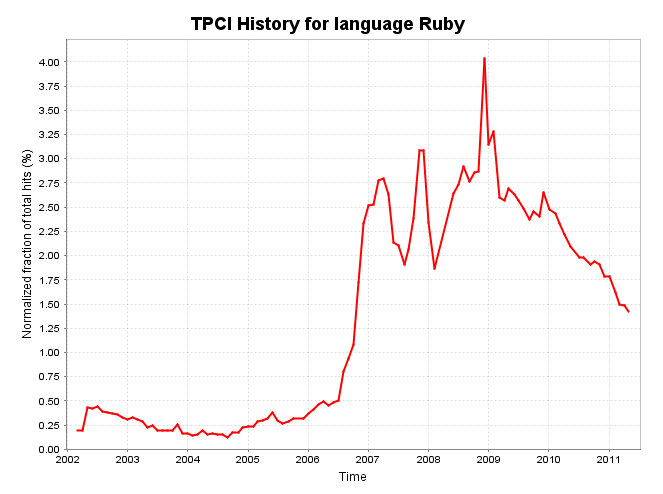
\includegraphics[width=425px]{TIOBE_ruby.png}\\
Quelle: www.tiobe.com/index.php/paperinfo/tpci/Ruby.html, 2011.
\end{figure}


\chapter{Syntax}
Das folgende Kapitel beschäftigt sich mit der Ruby-Syntax. Aus Java bekannte Elemente werden zwar angesprochen, jedoch wird nur kurz auf sie eingegangen. Dennoch ist dieses Kapitel wichtig um die späteren Beispiele und Konzepte besser zu verstehen.
 
\section{Kommentare}
Begonnen werden soll in diesem Kapitel mit einem kurzen Abschnitt über Kommentare. Kommentare beginnen in Ruby immer mit einem \texttt{\#}-Zeichen und setzen sich bis zum Zeilenende fort. 
Der Interpreter ignoriert das \texttt{\#}-Zeichen und jeglichen Folgetext, jedoch nicht den 'newline'-Character.\footcite[vgl.][S.26]{ruby_lang} Dieser dient in Ruby zudem als Anweisungsendmarkierung (zu vergleichen mit dem Semikolon ``\texttt{;}'' in Java, das in Ruby auch genutzt werden kann, aber meist weggelassen wird).\footcite[vgl.][S.32]{ruby_lang} Falls das \texttt{\#}-Zeichen hingegen innerhalb eines Strings oder eines regulären Ausdrucks steht, so leitet es keinen Kommentar ein, sondern ist einfach nur ein String, bzw. ein regulärer Ausdruck.
\inputminted[]{ruby}{comments.rb}
Kommentare über mehrere Zeilen werden einfach mit einem \texttt{\#} vor jeder Zeile realisiert. Es ist noch wichtig zu erwähnen, dass Ruby keine Inline-Kommentare (wie zum Beispiel \texttt{/* ... */} in Java oder C) unterstützt.\footcite[vgl.][S.26]{ruby_lang}


\section{Basisdatentypen}
Als nächstes werden die Basisdatentypen in Ruby behandelt. Dazu gehören \texttt{Integer}, wobei hier zwischen \texttt{Fixnum} und \texttt{Bignum} unterschieden wird, die beide Unterklassen von \texttt{Integer} sind, und \texttt{Float}. \texttt{Fixnum}-Objekte können ganze Zahlen bis zu einer Größe von 31 Bit darstellen. Sollte der Wertebereich darüber hinausgehen, so wird das \texttt{Fixnum} automatisch in ein \texttt{Bignum}-Objekt konvertiert. Die Begrenzung eines \texttt{Bignum}-Objektes liegt hierbei effektiv bei der Größe des zur Verfügung stehenden Speichers.\footcite[vgl.][S.315]{p_ruby}\\
Eine Zahl mit einem Dezimalpunkt und/oder einem Exponenten wird als \texttt{Float}-Objekt interpretiert. Dabei ist es wichtig zu beachten, dass mindestens eine Ziffer vor dem Dezimalpunkt steht und eine danach. Ist dies nicht der Fall (z.B. \texttt{1.e4}), so versucht Ruby die Methode \texttt{e4} an dem \texttt{Fixnum 1} aufzurufen.\footcite[vgl.][S.316]{p_ruby}\\
Zusätzlich existieren noch drei weitere Klassen zur Repräsentation von Zahlen: \texttt{Complex}, \texttt{BigDecimal} und \texttt{Rational}. Die Klassennamen sprechen in diesen Fällen für sich und geben gleichzeitig ihre jeweilige Funktion an. Übrigens sind in Ruby alle numerischen Objekte \textit{immutable}.\footcite[vgl.][S.42-43]{ruby_lang}
\begin{figure}[h]
\centering
\caption[\texttt{Numeric} Klassenhierarchie]{\texttt{Numeric} Klassenhierarchie}
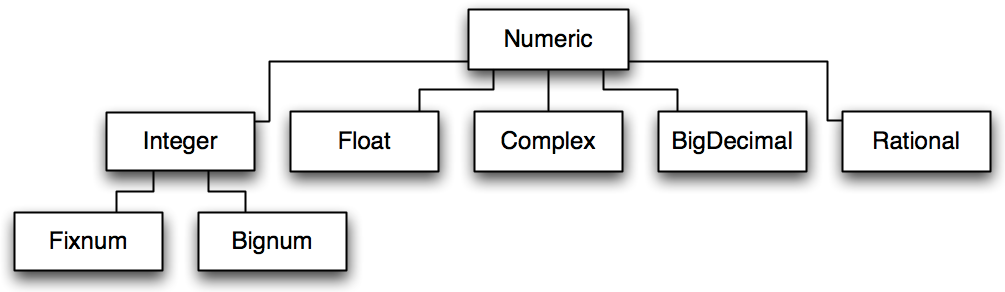
\includegraphics[width=400px]{numeric.png}
\end{figure}

Um Zeichenketten darzustellen gibt es auch in Ruby \texttt{String}s. Anders als in Java sind \texttt{String}-Objekte in Ruby \textit{mutable} und die \texttt{String}-Klasse bietet jede Menge Methoden um auf ihren Instanzen zu operieren. Strings können in einfache oder doppelte Anführungszeichen gesetzt werden, wobei Strings in doppelten Anführungszeichen wesentlich flexibler sind und einige Backslash-Escape-Sequenzen (wie z.B. $\backslash$\texttt{n} für Newline oder \texttt{$\backslash$t} für Tab) unterstützen. Strings in einfachen Anführungszeichen substituieren lediglich die Sequenz $\backslash \backslash$ in einen einzigen Backslash und $\backslash$\texttt{'} in ein Apostroph. Alle weiteren Escape-Sequenzen erscheinen unausgewertet in dem jeweiligen String.\footcite[vgl.][S.46-47]{ruby_lang}\footcite[vgl.][S.316-317]{p_ruby}
\inputminted[]{ruby}{basictypes.rb}
An diesem kleinen Beispiel lässt sich gut erkennen, das wirklich alles ein Objekt ist, selbst die Zahl \texttt{42}, an der die Methode \texttt{even?} aufgerufen werden kann. Dabei geschieht ein Methodenaufruf, genau wie in Java, über die bekannte Punktsyntax.\\
Als letzter Datentyp sollen die \texttt{Symbol}e vorgestellt werden. Sie beginnen stets mit einem Doppelpunkt gefolgt von einem Identifier oder einem String. Dabei können Anführungszeichen hilfreich sein, falls ein String durch Leerzeichen getrennt ist. Symbole können als ``konstante'' Strings verstanden werden (sie sind \textit{immutable}). Zwei normale Strings können zum Beispiel den gleichen Inhalt haben und dennoch zwei völlig verschiedene Objekte sein. Dies ist bei Symbolen nie der Fall. Zwei String-Symbole mit dem gleichen Inhalt werden beide zum selben \texttt{Symbol}-Objekt konvertiert. Folglich besitzen zwei verschiedene \texttt{Symbol}-Objekte immer einen unterschiedlichen Inhalt. In Ruby werden Symbole häufig bei \texttt{Hash}-Objekten verwendet, die im nachfolgenden Abschnitt erläutert werden. Zudem hält der Ruby-Interpreter eine \texttt{Symbol}-Tabelle vor, in der alle Klassennamen, Methoden und Variablen abgelegt werden, um die relativ teuren \texttt{String}-Vergleiche durch günstigere \texttt{Integer}-Vergleiche zu ersetzen.\footcite[vgl.][S.70-71]{ruby_lang}%\\
%\vspace{3mm}\\
%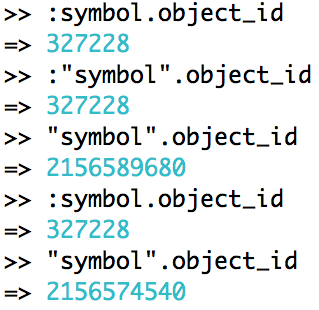
\includegraphics[width=140px]{symbol.png}
\inputminted[]{ruby}{symbol.rb}


\section{Arrays und Hashes}
Objekte der \texttt{Array}-Klasse werden erzeugt, indem man Objektreferenzen durch Kommata getrennt zwischen eckige Klammern schreibt. Ein nachstehendes Komma wird vom Interpreter ignoriert. Auf die jeweiligen Werte kann direkt über ihre Position, bzw. ihren Index (mit dem \texttt{[]}-Operator) zugegriffen werden. Die Methoden \texttt{size} und \texttt{length} liefern die Anzahl der Elemente des Arrays zurück. Des Weiteren sind Arrays dynamisch vergrößerbar. Weist man einen Wert einem Index jenseits der aktuellen Arraylänge zu, so wird das Array automatisch erweitert und mit \texttt{nil}-Elementen aufgefüllt. 
\footcite[vgl.][S.318]{p_ruby}
\inputminted[]{ruby}{arrays.rb}
Ein Objekt der Ruby \texttt{Hash}-Klasse wird durch das Setzen von Schlüssel/Wert-Paaren zwischen zwei geschwungene Klammern erzeugt und ist mit der Java \texttt{HashMap} zu vergleichen. Einem Schlüssel wird dabei durch einen Pfeil (\texttt{=>}) ein Wert zugewiesen.
\footcite[vgl.][S.318-319]{p_ruby}
\inputminted[]{ruby}{hashes.rb}


\section{Operatoren}
\begin{figure}[h]
\centering
\caption[Operatoren in Ruby]{Operatoren in Ruby}
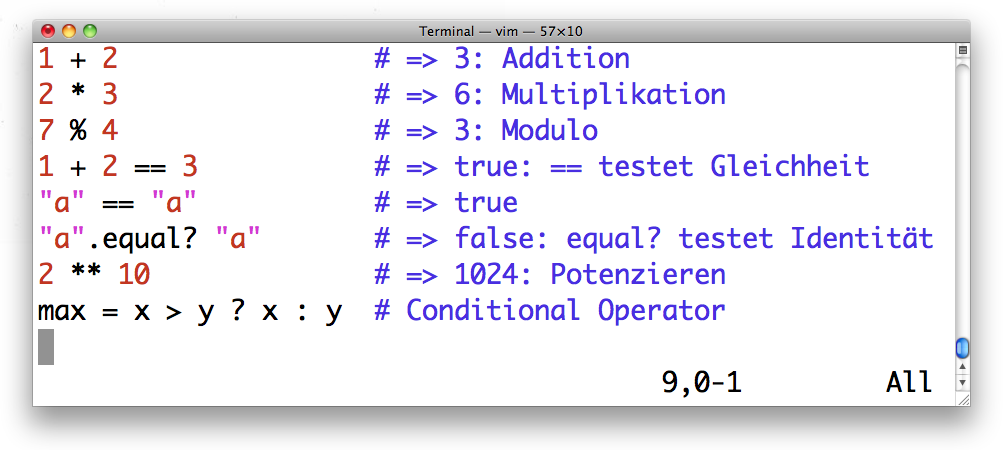
\includegraphics[width=425px]{operators.jpg}\\
Quelle: Thomas/Flower/Hunt (2009), S.333.
\end{figure}

%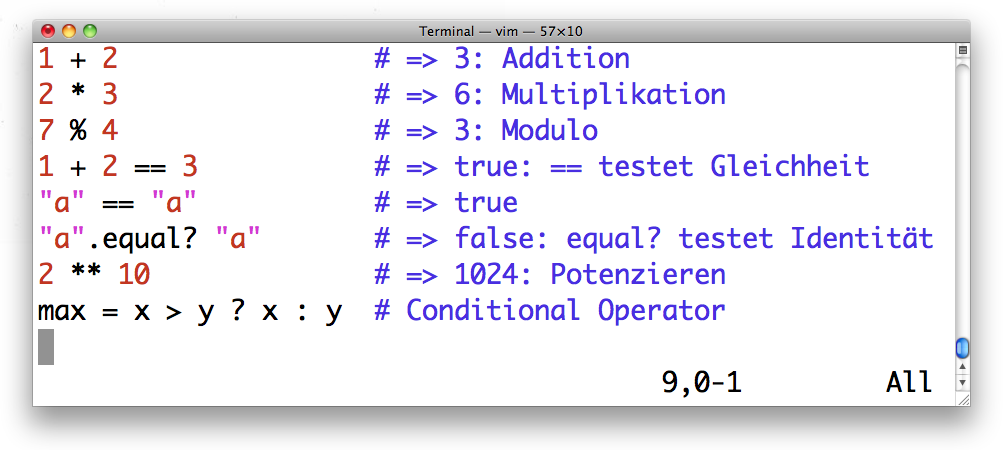
\includegraphics[width=450px]{operators.jpg}
Die oben stehende Tabelle ist eine Auflistung aller Operatoren in Ruby. In der Spalte ``Method'' sind die Operatoren gekennzeichnet, die als Methoden implementiert wurden und somit überschrieben werden können (ähnlich zu C++). Aufgrund der großen Überschneidungen zu Java soll im Folgenden nur auf einige wenige Operatoren näher eingegangen werden.\\
Im Gegensatz zu Java existiert in Ruby explizit der \texttt{**}-Operator zum Potenzieren. \texttt{2 ** 10} bedeutet also $2^{10}$. Ebenfalls interessant ist der \texttt{===}-Operator, auch Case-Equality-Operator genannt, da er implizit bei \texttt{case}-Anweisungen genutzt wird. Er prüft auf Zugehörigkeit (Membership) oder auf Muster (Pattern-Matching).\footcite[vgl.][S.106]{ruby_lang}\\
Einen direkten Inkrementierungs- bzw. Dekrementierungs-Operator (wie z.B. \texttt{++} oder \texttt{--} in Java) gibt es in Ruby nicht.

\subsection{Zuweisungen}
Wie aus der Tabelle ersichtlich ist, lassen sich die Zuweisungsopreatoren nicht überladen bzw. überschreiben. Eine Besonderheit, die hier allerdings herausgestellt werden soll ist die parallele Zuweisung mehrerer Werte.\\
Besitzt eine Zuweisung mehr als einen Wert auf der linken Seite (lWerte), so gibt der Zuweisungsausdruck ein Array der Werte auf der rechten Seite (rWerte) zurück. Überwiegt die Anzahl der lWerte gegenüber den rWerten, dann werden die überschüssigen lWerte auf \texttt{nil} gesetzt. Sind im Gegensatz mehr rWerte vorhanden als lWerte, so werden die überschüssigen rWerte ignoriert. Werden mehrere rWerte einem einzigen lWert zugewiesen, so werden die rWerte seit Ruby 1.6.2 automatisch in ein Array umgewandelt.\\
Eine weitere Funktionalität bietet der \texttt{*}-Operator. Mit diesem lassen sich Arrays auf- und wieder zuklappen. Steht zum Beispiel vor dem letzten lWert ein Sternchen, so werden alle restlichen rWerte gesammelt und diesem lWert als ein Array zugewiesen. Ist der letzte rWert ein Array, dann kann diesem ein Sternchen vorangestellt werden, wordurch es in seine Elemente zerlegt wird und es möglich ist, diese einzeln zuzuweisen. Dies ist nicht nötig, wenn auf der rechten Seite nur ein Array steht. In diesem Fall erfolgt das Aufklappen automatisch.
\footcite[vgl.][S.97-100]{ruby_lang}
\inputminted[]{ruby}{zuweisungen1.rb}
Eine weitere Eigenschaft der parallelen Zuweisung ist die Verschachtelung. Dabei kann die linke Seite einer Zuweisung eine in Klammern gesetzte Liste von Termen enthalten. Diese werden von Ruby so behandelt, als seien es geschachtelte Zuweisungsanweisungen.
Der entsprechende rWert wird extrahiert und den in Klammern stehenden Termen zugewiesen, bevor mit der Zuweisung auf höherer Ebene fortgefahren wird.
\footcite[vgl.][S.134-135]{p_ruby}
\inputminted[]{ruby}{zuweisungen2.rb}

\subsection{\texttt{==} vs. \texttt{equal?}}
Für den Java-Programmierer zunächst etwas gewöhnungsbedürftig dürfte die Verwendung des \texttt{==}-Operators sein. Dieser prüft in Ruby nämlich auf inhaltliche und nicht auf Referenzengleichheit. Dafür gibt es in Ruby die \texttt{equal?}-Methode, die die jeweilige \texttt{object\_id} zweier Objekte miteinander vergleicht.\footcite[vgl.][S.76]{ruby_lang}
\inputminted[]{ruby}{equal.rb}

\subsection{Range}
Ein \texttt{Range}-Objekt repräsentiert die Werte zwischen einem Start- und einem Endwert. Erzeugt werden sie durch das Schreiben von zwei bzw. drei Punkten zwischen dem Start- und dem Endwert (also \texttt{..} bzw. \texttt{...}). Zwei Punkte bedeuten, dass der Endwert noch in der Range enthalten ist (inklusive), bei drei Punkten ist der Endwert nicht mehr Teil der Range (exklusive).\footcite[vgl.][S.68-70]{ruby_lang} 
Deutlich wird dies im unteren Beispiel, in dem nun auch der \texttt{===}-Operator zum Einsatz kommt.
\inputminted[]{ruby}{range.rb}

\section{Reguläre Ausdrücke}
Wie auch in anderen Sprachen gibt es in Ruby Reguläre Ausdrücke (oder auch \texttt{Regexp}). Sie bieten eine komfortable Möglichkeit Pattern-Matching auf Strings durchzuführen. In der Praxis werden reguläre Ausdrücke meist dazu verwedet, um zu testen, ob ein String einem bestimmten Muster entspricht, Teile aus einem String zu extrahieren, die einem Muster entsprechen oder Teile eines Strings zu ersetzen.\footcite[vgl.][S.99]{p_ruby}
Reguläre Ausdrücke werden durch zwei Slashes begrenzt. Zum Prüfen, ob ein String einem bestimmten Muster entspricht, wird der \texttt{=\~}-Operator benutzt.\footcite[vgl.][S.100]{p_ruby}\\
Da die Möglichkeiten mit Regulären Ausdrücken zu arbeiten recht umfangreich sind, sollen hier nur einige wenige Beispiele dargestellt werden, um zu zeigen dass Ruby diese Funktionalität bietet. Wer sich intensiver mit den \texttt{Regexp} beschäftigen möchte, wird in der angegebenen Literatur fündig.\\
Zur Veranschaulichung seien hier die eckigen Klammern genannt, die ihre beinhaltenden Character mit einem logischen ``oder'' verknüpfen. Es gibt zusätzlich vorgefertigte Character-Klassen wie z.B. \texttt{/$\backslash$d/}, die testet, ob ein String eine Ziffer enthält. Möchte man wissen, ob ein String mit \texttt{y} oder \texttt{Y} beginnt, so testet man mit \texttt{/\^{}[yY]/}.\footcite[vgl.][S.310-321]{ruby_lang}
\inputminted[]{ruby}{regexp1.rb}


\section{Methoden und Variablen}
 Nachdem die Grundlagen der Ruby-Syntax behandelt wurden, geht es nun weiter zu den nächst komplexeren Gebilden, den Methoden.\\
Methoden werden in Ruby durch das Schlüsselwort \texttt{def} eingeleitet, gefolgt von dem Methodennamen und den formalen Parametern in Klammern (Klammern können weggelassen werden, aber nach Konvention nur, wenn keine Parameter an die Methode übergeben werden). Durch das Schlüsselwort \texttt{end} wird das Ende der Methode angezeigt.\footcite[vgl.][S.177]{ruby_lang}
Laut Konvention beginnen Methodennamen immer mit einem Kleinbuchstaben, da sie sonst mit Konstanten verwechselt werden können, und folgen dem \texttt{snake\_case} anstatt dem \texttt{camelCase}-Schema.\footcite[vgl.][S.180]{ruby_lang}
Methodennamen können, müssen aber nicht, mit einem Fragezeichen, einem Ausrufungszeichen oder einem Gleichheitszeichen enden. In jedem dieser Fälle ist für den Aufrufer der Methode eine bestimmte Funktionalität zu erkennen. Methoden, die mit einem \texttt{?} enden (z.B. \texttt{even?} oder \texttt{equal?}) liefern \texttt{true} oder \texttt{false} zurück. Methoden, die auf ein \texttt{!} enden, wobei zu diesen Methoden meist ein Pendant mit dem selben Namen ohne Ausrufungszeichen existiert, sind zum Beispiel \texttt{sort} und \texttt{sort!}. Die \texttt{sort}-Methode liefert ein modifiziertes Objekt zurück und arbeitet auf einer Kopie, die \texttt{sort!}-Methode hingegen operiert auf dem Originalobjekt. Methoden, die auf ein \texttt{=}-Zeichen enden fungieren als Setter-Methoden und können mit der Zuweisungssyntax aufgerufen werden. \footcite[vgl.][S.119-120]{p_ruby}
\\
Ein Methodenaufruf an einem Objekt geschieht mit Hilfe der (auch aus Java) bekannten Punktsyntax. Die Parameterübergabe folgt dem Prinzip ``Call by Value''.\footcite[vgl.][S.122]{p_ruby}\\
Der Rückgabewert einer Methode muss nicht explizit im Methodenkopf angegeben werden. Terminiert die Methode normal, so wird der letzte ausgewertete Ausdruck innerhalb des Rumpfes implizit zurückgeliefert (im unteren Beispiel würde also der \texttt{String ``überall sichtbar''} zurückgegeben). Es besteht weiterhin die Möglichkeit das Schlüsselwort \texttt{return} zu verwenden, welches allerdings meistens nur genutzt wird, um einen Wert vorzeitig an den Aufrufenden zurück zu liefern.\footcite[vgl.][S.177-178]{ruby_lang}

\inputminted[]{ruby}{method.rb}

Neben der Methodensyntax soll ebenfalls auf die vier unterschiedlichen Arten von Variablen eingegangen werden. Zunächst fällt auf, dass in Ruby auf Typdeklarationen vor Variablen verzichtet werden kann, da diese dynamisch typisiert werden.\footcite[vgl.][S.324]{p_ruby}
\\ 
Lokale Variablen beginnen mit einem Unterstrich oder einem Kleinbuchstaben und sind nur innerhalb des aktuellen Blocks oder der aktuellen Methode sichtbar.\footcite[vgl.][S.87]{ruby_lang} Variablen, die mit \texttt{@} oder \texttt{@@} beginnen sind Instanz-, bzw. Klassenvariablen.\footcite[vgl.][S.87]{ruby_lang}
Instanzvariablen werden so gekapselt, dass man nur über die Instanzmethoden des jeweiligen Objekts auf sie zugreifen kann.\footcite[vgl.][S.216]{ruby_lang}
Klassenvariablen sind in der gesamten Klasse sichtbar und werden von den Klassen-, sowie Instanzmethoden geteilt. Sie sind zu vergleichen mit \texttt{static}-Variablen aus Java. Klassenvariablen werden ebenfalls gekapselt und sind für den Benutzer der Klasse nicht sichtbar.\footcite[vgl.][S.230]{ruby_lang}
Globale Variablen beginnen mit einem \texttt{\$}-Zeichen und sind überall sichtbar.\footcite[vgl.][S.87]{ruby_lang}\\
Weiterhin existieren in Ruby zusätzlich Konstanten. Diese beginnen mit einem Großbuchstaben und werden meist durchgängig groß geschrieben. Wird einer Konstante das erste Mal ein Wert zugewiesen, so sollte dieser konstant bleiben. In Ruby lassen sich die Werte von Konstanten im Programmverlauf allerdings ändern. Dieses Vorgehen ruft keinen Fehler hervor, sondern generiert lediglich eine Warnmeldung durch den Interpreter. Aus diesem Grund werden die Konstanten unter der Rubrik Variablen mit aufgeführt.\footcite[vgl.][S.324]{p_ruby}\\
Zuletzt seien noch die Methodensichtbarkeiten angesprochen, die mit sogenannten Modifiern gesteuert werden können. Die drei unterschiedlichen Sichtbarkeitstypen werden mit \texttt{public}, \texttt{private} und \texttt{protected} betitelt. Methoden sind von Natur aus \texttt{public}, außer sie werden explizit als \texttt{private} oder \texttt{protected} deklariert. Eine Ausnahme bildet hier die \texttt{initialize}-Methode, die stets implizit \texttt{private} ist (s. Abschnitt ``Klassen''). Ist eine Methode \texttt{protected}, so kann diese von jeder Instanz der definierenden oder einer erbenden Klasse aufgerufen werden. Falls eine Methode als \texttt{private} deklariert ist, so kann sie nur innerhalb des aufrufenden Objekts benutzt werden. Es ist nicht möglich direkt auf private Instanzmethoden anderer Objekte zuzugreifen, selbst, wenn es ein Objekt der selben Klasse ist. Dennoch sind private Methoden für vererbte Klassen sichtbar. Folglich ist es in Ruby nicht möglich Methoden komplett zu verstecken. Für den Aufruf einer privaten Methode \texttt{method} bedeutet dies konkret, dass man sie wie eine Funktion ohne konkreten Empfänger aufrufen muss, also nur \texttt{method}. Man kann weder \texttt{object.method}, noch \texttt{self.method} schreiben.\footcite[vgl.][S.232-234]{ruby_lang}


\section{Klammern}
Eine weitere Besonderheit von Ruby sind die optionalen Klammern bei Methodenaufrufen und konditionalen Ausdrücken (im Gegensatz zu Java). Die Regel lautet hier, dass die Klammern in einfachen Fällen und bei Eindeutigkeit weggelassen werden können.\footcite[vgl.][S.124]{p_ruby} Das Ergebnis ist sauberer und klarer Code. In komplexeren Fällen und bei Verwirrungsgefahr sollte man Klammern um jeden Preis nutzen, da es sonst schnell zu syntaktischer Unklarheit kommen kann.\footcite[vgl.][S.183]{ruby_lang}\\
In dem unteren Beispiel wird jeweils die Variante mit und ohne Klammern aufgeführt. Bei Methoden, denen ein Hash übergeben wird, können zusätzlich zu den runden, sogar die geschwungenen Klammern weggelassen werden.

\inputminted[]{ruby}{klammern.rb}


\section{Kontrollstrukturen}
Wie in jeder Sprache gibt es auch in Ruby gewisse Kontrollstrukturen, um den Programmfluss zu verzweigen, Codeteile nur unter bestimmten Voraussetzungen auszuführen oder zu wiederholen. Vorweg ist es noch wichtig zu erwähnen, dass in Ruby jeder Wert wie \texttt{true} behandelt wird, außer \texttt{false} und \texttt{nil}. Dies sollte man bei der Verwendung von Kontrollstrukturen im Hinterkopf behalten.\footcite[vgl.][S.11]{ruby_lang}

\subsection{Bedingte Anweisungen und Verzweigung}
Die wohl geläufigste bedingte Anweisung ist die \texttt{if}-Anweisung. Diese funktioniert in Ruby ähnlich wie in Java.\footcite[vgl.][S.337]{p_ruby}
\inputminted[]{ruby}{if1.rb}
Die offensichtlichen Unterschiede sind zum einen die fehlenden Klammern um die Bedingung sowie der Abschluss des Statements mit \texttt{end} anstatt geschweiften Klammern. Möchte man eine Mehrfachverzweigung realisieren, so nutzt man \texttt{elsif} um weitere Bedingungen zu prüfen und \texttt{else} für alle anderen Fälle. Mit einem \texttt{then} ist es zudem möglich die Anweisung in die selbe Zeile zu schreiben in der auch die Bedingung steht.\footcite[vgl.][S.118-122]{ruby_lang}\\
Die \texttt{unless}-Anweisung bildet das Gegenteil zu \texttt{if}, da der \texttt{body} nur ausgeführt wird, wenn der \texttt{boolean\_expression} als \texttt{false} oder \texttt{nil} ausgewertet wird.\footcite[vgl.][S.122-123]{ruby_lang}
Die Funktionsweise wird im Folgenden gezeigt.\footcite[vgl.][S.337]{p_ruby}
\inputminted[]{ruby}{unless.rb}

Anstatt nun einzeilige Bedingungen  mit \texttt{then} und \texttt{end} schreiben zu müssen, können \texttt{if} und \texttt{unless} auch als Modifier genutzt werden.\\
Dabei wird der \texttt{expression} nur ausgewertet, falls \texttt{boolean\_expression} \texttt{true} (für \texttt{if}) oder \texttt{false} (für \texttt{unless}) ist.\footcite[vgl.][S.337]{p_ruby}
\inputminted[]{ruby}{if_unless.rb}

Des Weiteren verfügt Ruby über eine \texttt{case}-Anweisung, die üblicherweise wie folgt eingesetzt wird:
\inputminted[]{ruby}{case1.rb}
Hier kommt nun der zuvor schon angesprochene Case-Equality-Operator \texttt{===} implizit beim Vergleichen zum Einsatz. Es wird eine Übereinstimmung des \texttt{target} mit einem der \texttt{when}-Fälle geprüft (\texttt{comparison === target}) und entsprechend abgearbeitet.\footcite[vgl.][S.338]{p_ruby}

\subsection{Schleifen}
Neben den Bedingten Anweisungen existieren in Ruby die Schleifen. Dazu gehören die \texttt{while}- und die \texttt{until}-Schleife. Diese führen den Code in ihrem Rumpf aus, solange (\texttt{while}) eine bestimmte Bedingung \texttt{true} ist oder bis (\texttt{until}) diese Bedingung  \texttt{true} wird. Die Syntax der beiden Schleifen ergibt sich wie folgt:\footcite[vgl.][S.338]{p_ruby}
\inputminted[]{ruby}{while.rb}
\inputminted[]{ruby}{until.rb}
Ebenso wie \texttt{if} und \texttt{unless} können auch \texttt{while} und \texttt{until} als Modifier genutzt werden:
\inputminted[]{ruby}{while_until.rb}

\subsection{Blöcke und Iteratoren}
Blöcke und Iteratoren nehmen eine Sonderstellung ein und beschreiben eine von Rubys besonderen Stärken. Es ist möglich Code-Blöcke an Methoden zu übergeben, fast so als wären es Parameter. Dabei bestehen Code-Blöcke lediglich aus Code, der zwischen zwei geschweiften Klammern oder einem \texttt{do/end}-Konstrukt steht. Hierbei muss die öffnende geschwungene Klammer bzw. das \texttt{do} immer in der selben Zeile stehen wie der Methodenaufruf. Die Konvention schreibt vor, die geschwungenen Klammern bei einzeiligen und das \texttt{do/end} bei mehrzeiligen Blöcken zu benutzen.\footcite[vgl.][S.24]{p_ruby}\\
Grundsätzlich können Blöcke nicht allein stehen und treten nur in Verbindung mit einem Methodenaufruf auf. Prinzipiell kann ein Block nach jeder beliebigen Methode stehen. Ist diese allerdings weder ein Iterator noch ruft sie den Block mit \texttt{yield} auf, so wird der Block nicht weiter beachtet.\footcite[vgl.][S.141]{ruby_lang}
Blöcke können Parameter enthalten, die, anders als bei Methoden, in vertikalen Strichen (z.B. \texttt{|x|}) stehen müssen. So wird bei der \texttt{each}-Methode im unteren Beispiel für jedes Element aus der \texttt{Range (1..10)} die Quadratzahl ausgegeben. Dabei wird intern eine Schleife generiert und (in unserem Fall) das \texttt{i} durch die jeweilige Zahl ersetzt. Der Code-Block wird also für jedes Element des aufrufenden Objektes einmal ausgeführt.\footcite[vgl.][S.56]{p_ruby}
\inputminted[]{ruby}{iterators.rb}
Die Methoden \texttt{times}, \texttt{upto} und \texttt{each} (und einige andere) sind Iteratoren und anhand ihres Names und der obigen Beispiele recht selbsterklärend. Diese Methoden können mit einem Code-Block als Parameter aufgerufen werden. Die Variante der Blöcke wird üblicherweise der normalen \texttt{while}-Schleife vorgezogen.\footcite[vgl.][S.3-4 und S.130]{ruby_lang}


\section{Klassen}
Der letzte Teil des Syntax-Kapitels befasst sich mit den Klassen, die in der objektorientierten Programmierung eine entscheidene Rolle spielen.
In Ruby werden Klassen mit dem Schlüsselwort \texttt{class} eingeleitet und enden mit dem Schlüsselwort \texttt{end}. Der Name einer Klasse muss immer mit einem Großbuchstaben beginnen.\footcite[vgl.][S.215]{ruby_lang} Klassen stellen eine Sammlung von Methoden dar, die auf dem Zustand eines Objektes operieren können. Dieser Objektzustand wird durch die Instanzvariablen repräsentiert.
\\
Anhand der folgenden Beispielklasse \texttt{Person} sollen die wesentlichen Bestandteile und Funktionalitäten von Klassen und bestimmten Methoden verdeutlicht werden. 
\inputminted[]{ruby}{person.rb}
Um Instanzen einer Klasse erstellen zu können, wird ein Konstruktor benötigt. Dieser heißt in Ruby immer \texttt{initialize} und wird mit \texttt{Person.new} aufgerufen.\footcite[vgl.][S.215-216]{ruby_lang} Es besteht die Möglichkeit den Variablen, die dem Konstruktor übergeben werden, direkt Default-Werte zuzuweisen. Auffällig ist, dass die Instanzvariablen unmittelbar initialisiert werden können ohne vorher deklariert zu werden (man beachte die Parallenzuweisung). In der ersten Zeile der Klasse Person wird die Methode \texttt{attr\_accessor} aufgerufen, die sehr praktisch ist, da sie automatisch Getter- und Setter-Methoden für alle nachstehenden Instanzvariablen erstellt. Die Getter-Methoden haben dann die gleichen Namen wie die zugehörigen Instanzvariablen (in diesem Fall werden also die drei Methoden \texttt{name}, \texttt{age} und \texttt{footsize} erstellt). Die Setter-Methoden heißen ebenfalls so wie die entsprechenden Instanzvariablen mit dem Zusatz ``\texttt{=}'' am Ende des Namens (hier folglich \texttt{name=}, \texttt{age=} und \texttt{footsize=}). Der Aufruf der Setter-Methoden kann zum einen mit \texttt{name=} und zum anderen mit \texttt{name =} (mit Leerzeichen) geschehen. Diese Hilfsmethode erspart einem somit viel Schreibarbeit und Zeit. Möchte man lediglich lesenden Zugriff auf die Instanzvariablen gewähren, so benutzt man \texttt{attr\_reader}, um nur Getter erstellen zu lassen.\footcite[vgl.][S.218-219]{ruby_lang}\\
Wie auch in Java verfügt jedes Objekt über eine geerbte \texttt{toString()}-Methode, die in Ruby einfach nur \texttt{to\_s} heißt. Diese wird in dem Beispiel überschrieben. Interessant daran ist das Einfügen von Variablen in einen String. Dies geschieht mit Hilfe von \texttt{\#\{expression\}}. Dabei wird die Variable, oder der Ausdruck in den geschweiften Klammern ausgewertet und zu einem String substituiert.\footcite[vgl.][S.90-91]{p_ruby}


\chapter{Konzepte}
Nachdem im vorherigen Kapitel das Thema Grundlagen abgeschlossen wurde, widmet sich dieses Kapitel nun einigen Konzepten, die Ruby unterstützt. Dazu gehören die Module, Vererbung, Duck-Typing und das Metaprogramming, wobei letzteres nur sehr kurz thematisiert wird.

\section{Module}
Module können ebenso wie Klassen Methoden, Konstanten und Klassenvariablen beinhalten. Definiert werden sie ebenfalls wie Klassen, allerdings mit den Schlüsselwort \texttt{module} anstatt \texttt{class}. Zudem können Module nicht instanziiert werden und man kann nicht von ihnen erben. Das bedeutet, dass Module für sich allein stehen und es keine Modulhierarchie oder ähnliches gibt.\\
So wie ein \texttt{class}-Objekt eine Instanz der Klasse \texttt{Class} ist, so ist ein \texttt{module}-Objekt eine Instanz der Klasse \texttt{Module}. Hierbei ist \texttt{Class} eine Unterklasse von \texttt{Module}. Das bedeutet, dass alle Klassen Module sind, aber nicht alle Module Klassen. Module mit Modulmethoden bilden Namespaces, ebenso wie Klassen mit Klassenmethoden. Module mit Instanzmethoden werden als Mixins benutzt, wobei eine Klasse niemals als ein solches fungieren kann.\footcite[vgl.][S.247-248]{ruby_lang}\\
Im weiteren Verlauf soll etwas näher auf Module als Namespaces bzw. Mixins eingegangen werden.

\subsection{Module als Namespace}
Module bieten eine gute Möglichkeit verwandte Methoden zu gruppieren, wenn objektorientiertes Programmieren nicht notwendig ist. Als ein Ruby-internes Beispiel sei das \texttt{Math}-Module genannt, welches als Namespace fungiert und viele mathematische Funktionen bereitstellt (z.B. \texttt{Math.sqrt(9)} liefert \texttt{3}).\footcite[vgl.][S.248]{ruby_lang}
\inputminted[]{ruby}{namespace.rb}
Das obere Beispiel zeigt einen selbst definierten Namespace. Wichtig ist hierbei, dass nur Modulmethoden bzw. Klassenmethoden implementiert werden dürfen. Erwirkt wird dies durch den Modul- bzw. Klassennamen \texttt{Mein\_Modul} oder das Schlüsselwort \texttt{self} gefolgt von einem Punkt und dem Methodennamen. \footcite[vgl.][S.248-249]{ruby_lang}
Der Aufruf einer Modul- oder Klassenmethode erfolgt einfach durch Nennung des Modul- bzw. Klassennamens, einem Punkt und der entsprechenden Methode.

\subsection{Module als Mixins}
Die alternative Verwendung von Modulen sind die sogenannte Mixins, die mächtiger sind als die Namespaces. Sie sind zu vergleichen mit den Interfaces in Java. Definiert ein Modul Instanzmethoden anstatt Klassenmethoden, so können diese Instanzmethoden in andere Klassen hineinge\texttt{mix}t werden (daher der Name). Sehr bekannt sind zum Beispiel das \texttt{Enumerable} oder das \texttt{Comparable} Mixin. Anders als bei den Java-\texttt{Interfaces} können die Instanzmethoden der Mixins Code enthalten und diesen anderen Klassen zur Verfügung stellen. Dies wird durch die \texttt{include}-Methode realisiert, wobei eine beliebige Anzahl von Mixins angegeben werden kann.\footcite[vgl.][S.250-251]{ruby_lang}
\inputminted[]{ruby}{mixin.rb}
Auch hier soll ein kleines Beispiel zur besseren Veranschaulichung dienen. \texttt{Mein\_Modul} besitzt eine Instanzmethode \texttt{meine\_methode}. \texttt{Meine\_Klasse} bindet \texttt{Mein\_Modul} als Mixin ein und der Aufruf der Methode \texttt{meine\_methode} von einem neuen \texttt{Meine\_Klasse}-Objekt liefert den Output \texttt{Hello!}. 

\section{Vererbung}
Das Thema Vererbung wurde bereits angesprochen und wird in diesem Abschnitt etwas weiter vertieft. Das Prinzip der Vererbung ist aus den meisten objektorientierten Sprachen bereits bekannt, weshalb nur auf die wesentlichen Dinge eingegangen werden soll.\\
Alle Klassen in Ruby erben implizit von der Basisklasse \texttt{Object} (seit Ruby 1.9 von \texttt{BasicObject}). Somit werden jeder Klasse bereits einige Funktionalitäten zur Verfügung gestellt (z.B. die \texttt{to\_s}-Methode).\\
Um eine Klasse von einer anderen erben zu lassen schreibt man ein \texttt{$<$} in der Klassendefinition zwischen den Namen der erbenden und der vererbenden Klasse.\\
In Ruby gibt es keine direkte Mehrfachvererbung. Dennoch kann diese mit Hilfe von Mixins simuliert werden (warum das so ist wird im Kapitel Duck-Typing deutlich).\footcite[vgl.][S.71-77]{p_ruby} Geerbte Methoden können einfach überschrieben werden, z.B. um ihre Funktionalität anzupassen oder zu erweitern. Manchmal kann es sein, dass man eine Methode nicht gänzlich überschreiben möchte, sondern lediglich etwas Code hinzufügen will. Mit dem Schlüsselwort \texttt{super} lässt sich die überschriebene Methode von der überschreibenden Methode aufrufen. Dieses Prinzip nennt sich Chaining. \texttt{super} kann genutzt werden um Methoden oder Konstruktoren der Oberklasse aufzurufen. Grundsätzlich wird in Ruby alles an die Subklasse vererbt, also Instanzmethoden, private Methoden, Klassenmethoden, Instanzvariablen, Klassenvariablen und Konstanten.\footcite[vgl.][S.234-241]{ruby_lang}
\inputminted[]{ruby}{student.rb}
Die Beispielklasse \texttt{Person} wird nun durch die Klasse \texttt{Student} spezialisiert, indem \texttt{Student} von \texttt{Person} erbt. Es kommt die Instanzvariable \texttt{matrikel} neu hinzu. Um nun nicht den gesamten Konstruktor neu schreiben zu müssen, wird mit \texttt{super} der Konstrukter von \texttt{Person} aufgerufen und lediglich \texttt{@matrikel} in dieser Klasse gesetzt. Die \texttt{to\_s}-Methode wird ebenfalls überschrieben, allerdings so, das sie lediglich erweitert wird, weshalb erneut mit \texttt{super} die \texttt{to\_s}-Methode von \texttt{Person} aufgerufen wird.

\section{Duck-Typing}
Der Begriff Duck-Typing leitet sich von einem Gedicht von James Whitcomb Riley ab: \textit{``When I see a bird that walks like a duck and swims like a duck and quacks like a duck, I call that bird a duck.''}\\
Duck-Typing bietet ein Gegenkonzept zu typisierten Sprachen. Es ist weniger eine Menge von Regeln, sondern vielmehr ein Programmierstil. Duck-Typing sagt aus, dass ein Objekt in Abhängigkeit seiner Funktionalität (implementierte Methoden) behandelt wird und nicht in Abhängigkeit seines Typs. Das bedeutet, dass die Klassenzugehörigkeit eines Objektes egal ist, solange es die Methoden zur Verfügung stellt, die benötigt werden. Folglich ist nicht der Typ, sondern die bereitgestellte Funktionalität entscheidend. Nun wird nochmals deutlicher, weshalb mit Mixins eine Mehrfachvererbung sehr gut simuliert werden kann, denn letztlich ist es egal von welchem Typ ein Objekt ist, solange es die Methoden implementiert (evtl. auch durch Mixins), die gebraucht werden.\\
Das Prinzip des Duck-Typings spaltet die Programmierer in zwei Lager: Befürworter und Gegner. Manche mögen diese Art der Flexibilität und fühlen sich wohl dynamisch typisierten Code zu schreiben und andere (besonders C++ oder Java-Programmierer) können sich nicht vorstellen mit Ruby ernsthafte Applikationen zu schreiben.\footcite[vgl.][S.359-372]{p_ruby}
Verdeutlicht werden soll das Konzept Duck-Typing an einem einfachen Beispiel.
\inputminted[]{ruby}{schaf.rb}
Zunächst erstellen wir zwei Klassen: \texttt{Schaf} und \texttt{WolfImSchafspelz}. Beide besitzen die gleichen Methoden: \texttt{sag\_was} und \texttt{wer\_bist\_du}. Nun gibt es eine \texttt{schafstest}-Methode, die prüfen soll, ob das übergebene Objekt wirklich ein Schaf ist (allerdings nur mit einem String-Vergleich und nicht mit \texttt{instance\_of?}). Aufgrund der dynamischen Typisierung von Variablen ist es der Methode zunächst egal, was für einen Objekttyp sie übergeben bekommt, solange dieses die Methoden \texttt{sag\_was} und \texttt{wer\_bist\_du} zur Verfügung stellt. Da nun auch der \texttt{WolfImSchafspelz} in seiner Methode \texttt{wer\_bist\_du} den String \texttt{Ein Schaf} zurückliefert, ist die Ausgabe bei beiden Tests \texttt{Das ist wirklich ein Schaf}.\\
Für Java-Programmierer ist diese Möglichkeit zunächst sehr ungewöhnlich und vermittelt den Eindruck von Uneindeutigkeit, Verwirrung und evtl. Unsicherheit, doch in der Praxis scheint sich dieses Prinzip bewährt zu haben.

\section{Metaprogramming}
Was ist Metaprogramming? Metaprogramming bedeutet, wie der Name schon suggerieren lässt, auf einer höheren Abstraktionsebene zu arbeiten. Man ist nicht mehr durch die Abstraktionen der Programmiersprache eingeschränkt, sondern erschafft neue Abstraktionen, die in die Ursprungssprache integriert werden. Das heißt, man schreibt Code, der dabei hilft neuen Code zu schreiben oder zu generieren.
Des Weiteren erlaubt Metaprogramming das Ändern von Code bzw. Sprachkonstrukten (wie z.B. Klassen, Modulen, Instanzvariablen) zur Laufzeit. Es ist sogar möglich, Code zur Laufzeit zu schreiben und auszuführen, ohne das Programm neu starten zu müssen.\footcite[vgl.][S.373-408]{p_ruby}\\
So interessant dieses Konzept auch ist, so umfangreich ist es. Da dies allerdings nur eine Einführung in die Programmiersprache Ruby ist und es den Rahmen dieser Arbeit sprengen würde, soll das Thema Metaprogramming an dieser Stelle nicht weiter vertieft werden. Interessenten können sich allerdings in der weiterführenden Literatur einlesen.


\chapter{Fazit}
Man kann sich nun die Frage stellen, wofür Ruby überhaupt benötigt wird. In der Tat ist es so, dass eher selten Applikationen allein mit Ruby erstellt werden. Viel häufiger ist es der Fall, dass Ruby in Verbindung mit dem Framework Rails zum Einsatz kommt und damit ein sehr mächtiges Werkzeug für die Entwicklung von Web- oder Datenbankapplikationen zur Verfügung stellt, den Hauptanwendungsgebieten von Ruby.\\
Trotzdem ist die Sprache nicht zu unterschätzen. Neben dem in dieser Arbeit Gezeigten können in Ruby auch C- oder Java-Bibliotheken eingebunden oder GUI-Programme erstellt werden. Ruby bietet wirklich eine große Bandbreite an Möglichkeiten. Die Sprache ist, besonders im Empfinden von Java- oder C-Programmierern, sehr dynamisch, bietet aber gleichzeitig einen leichten Einstieg aufgrund der schnell zu erlernenden Syntax und Grammatik. Da das POLS (Principle of least surprise), also das Prinzip der geringsten Überraschung unterstützt wird\footcite[vgl.][S.486]{ruby}, ist Ruby in den meisten Fällen sehr intuitiv in der Anwendung.\\
Die zur Verfügung stehende, aktuelle Literatur ist leicht verständlich und gut geschrieben. Es existiert eine große und aktive Community, was zum Vorteil hat, dass man bei der Suche im Internet schnell auf viele Tutorials und Beispiele trifft. Weitere Pluspunkte sind die Plattformunabhängigkeit, die große API sowie die gute und umfangreiche Dokumentation.\footcite{ruby_doc}
Abschließend lässt sich sagen, dass es Spaß gemacht hat, sich in diese Programmiersprache einzuarbeiten, die unterhaltsame Literatur zu lesen und Ruby selbst zu schreiben und auszuprobieren. 
\newpage
\singlespacing

\bibliography{literatur}
\bibliographystyle{jurabib}

\end{document}
